\documentclass[a4paper, 12pt]{article}

\usepackage{wrapfig}
\usepackage{graphicx}
\usepackage{mathtext}
\usepackage{amsmath}
\usepackage{siunitx}
\usepackage{multirow}
\usepackage{rotating}

\usepackage[T1,T2A]{fontenc}

\usepackage[russian]{babel}

\graphicspath{{pictures/}}

\title{ \begin{center}Лабораторная работа №1.3.4\end{center}
ИССЛЕДОВАНИЕ СТАЦИОНАРНОГО ПОТОКА ЖИДКОСТИ В ТРУБЕ }
\author{Иванов И. И.}
\date{\today}

\usepackage[left=1.2cm,right=1.2cm,
    top=1.7cm,bottom=1.7cm,bindingoffset=0cm]{geometry}
\begin{document}

\maketitle
\newpage

\section{Введение}

\textbf{Цель работы:}
\begin{itemize}
    \item измерить скорости течения по методам Пито и Вентури, сравнить результаты со скоростью, определенной по расходу воды.
    \end{itemize}
\paragraph{}
\textbf{Оборудование:}
\begin{itemize}
    \item расходомерная установка; 
    \item линейка; 
    \item штангенциркуль;  
    \item секундомер.    
    \end{itemize}
\paragraph{}
В данной лабораторной работе мы определим среднюю скорость течения по прямолинейному участку трубы разными способами, а также вычислим числа Рейнольдса для оценки характера течения.
Рассмотрим используемую нами установку (см. рис. 1). Она состоит из цилиндрического резервуара $I$ с водоизмерительной трубкой $B$, куда поступает вода из водопровода по трубе $A$. Из резервуара вода попадает в трубу $T$, а из нее - в приемный резервуар $II$, имеющий сифон $C$, предотвращающий переполнение. Труба $T$ снабжена расходомерами Вентури и Пито (см. рис. 2).
Принцип их работы основан на уравнении Бернулли для несжимаемой жидкости ($\frac{P}{\rho} + \frac{v^2}{2} + gh = const$) и равенстве ($v_1S_1 = v_2S_2$) (формулы для определения скорости будут приведены в "Ходе работы").
\begin{figure}[h!]
        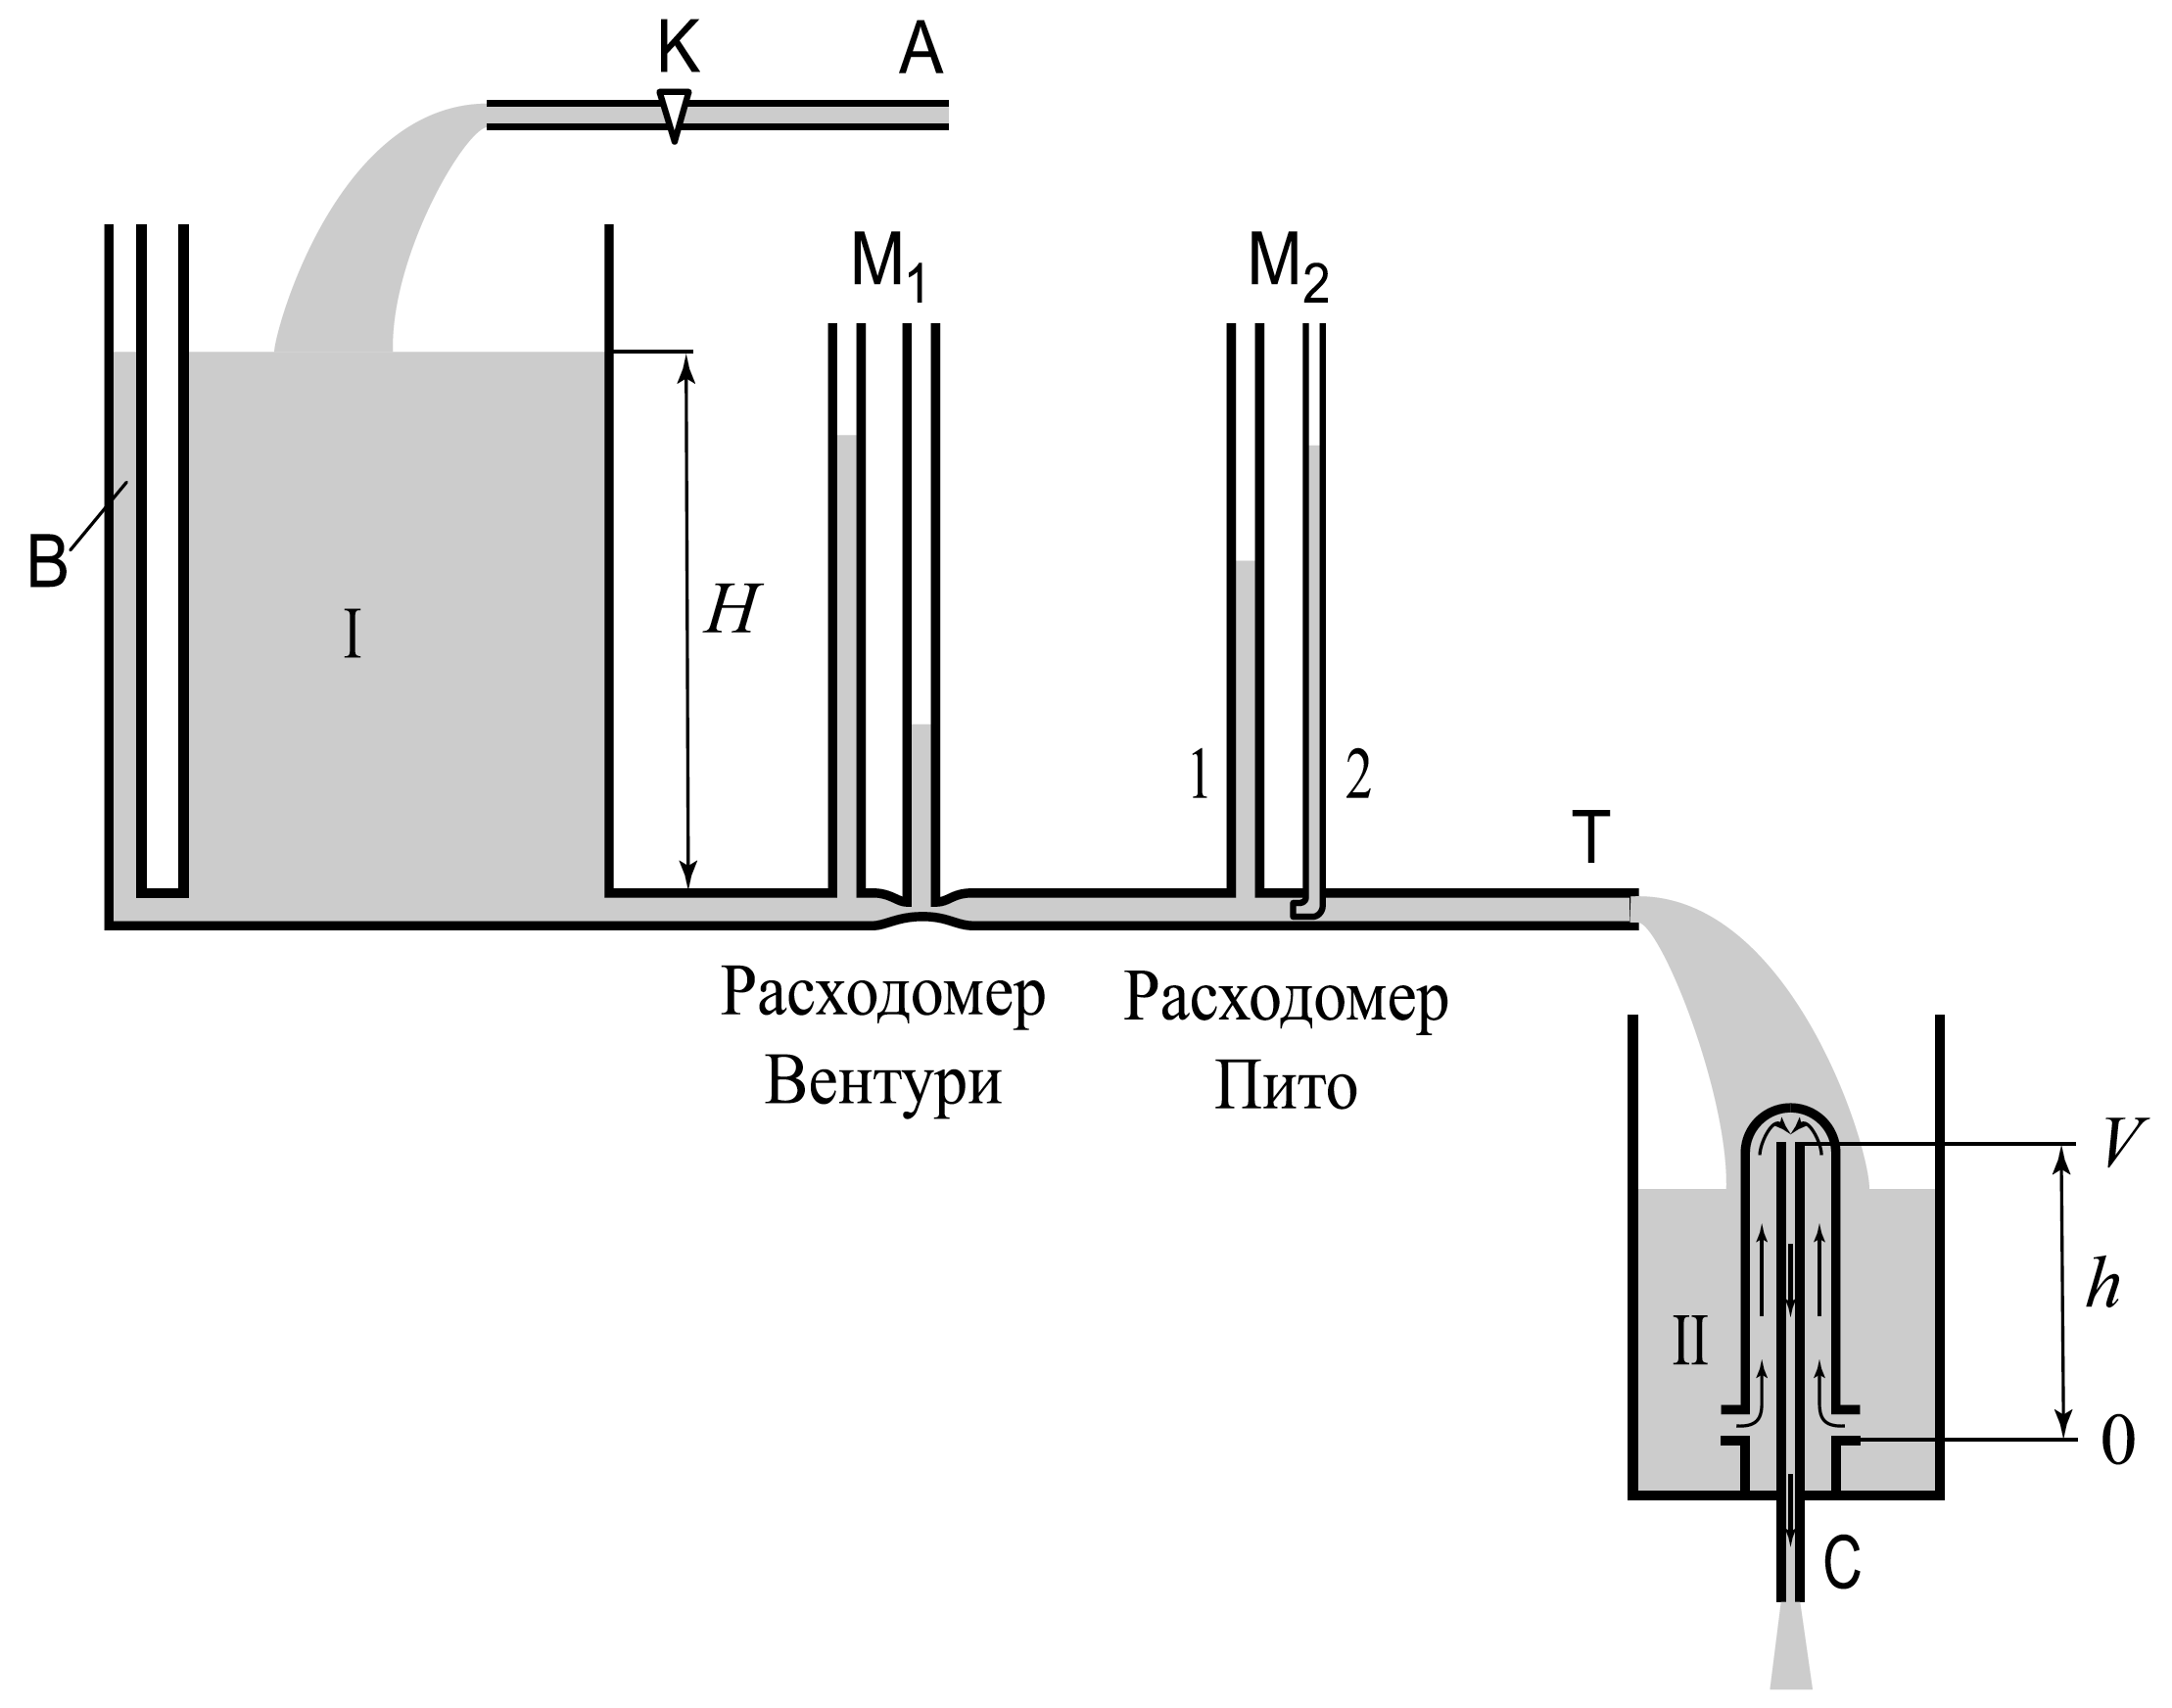
\includegraphics[width=0.8\textwidth]{ustanovka.png}
        \caption{Экспериментальная установка}
        \label{ris:ustanovka}
\end{figure}
\begin{figure}[h!]
        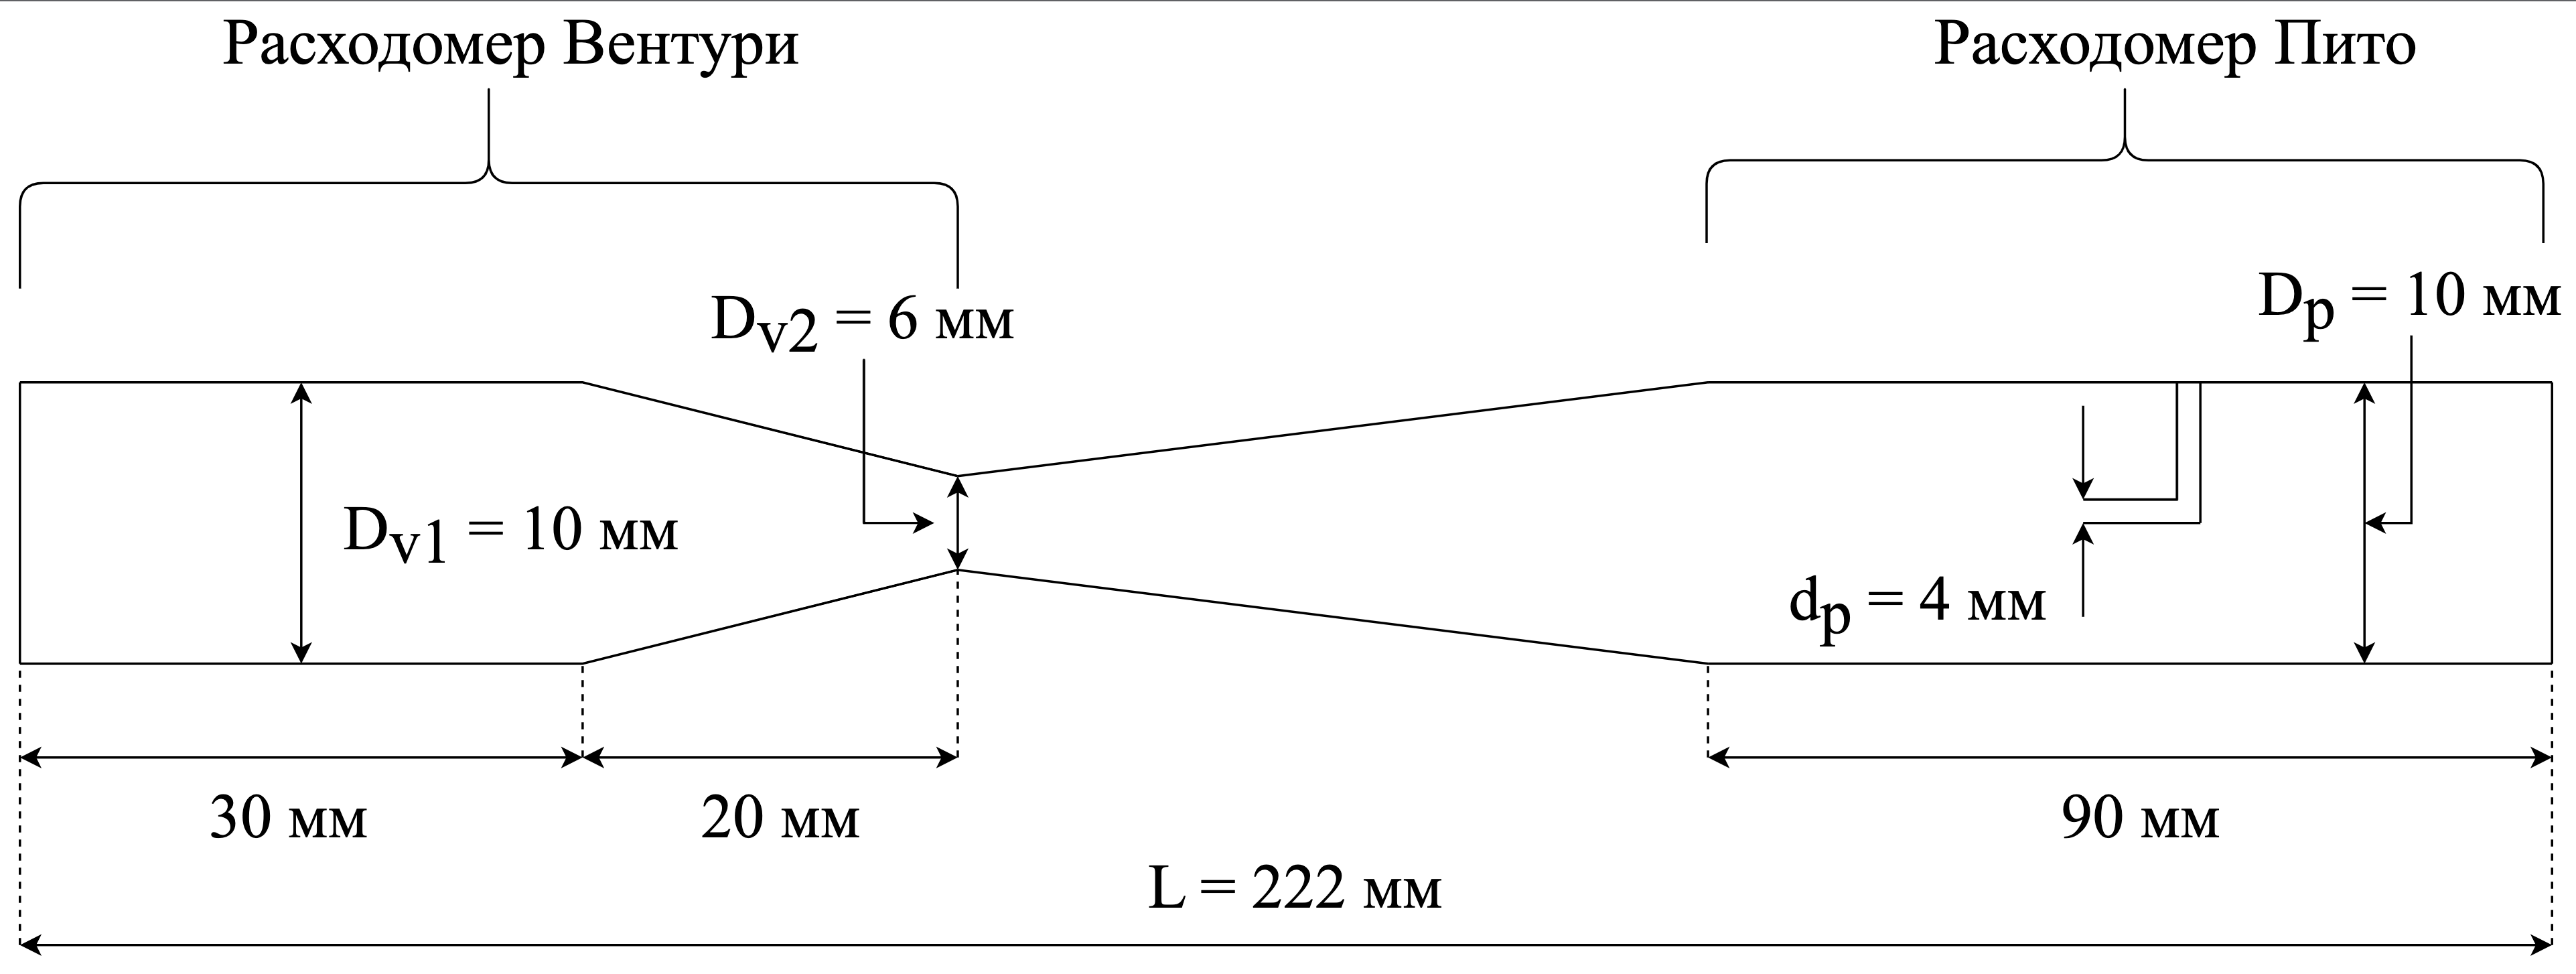
\includegraphics[width=1.0\textwidth]{pitovent.png}
        \caption{Размеры расходомеров Вентури и Пито на установке}
        \label{ris:ustanovka}
\end{figure}
\section{Ход работы}
\paragraph{Параметры установки}
\[ L = (222 \pm 1) \: мм \quad \Delta l = (20.00 \pm 0.05) \: мм \quad R_{v1} = R_p = (5.00 \pm 0.05)\: мм\quad R_{v2} = (3 \pm 0.05) \: мм \]\[\quad r_p = (2 \pm 0.05) \: мм \quad S_{бак} = (0.0390 \pm 0.0003) \: м^2
\quad \text{(длина трубы, расстояние между манометрами, }\]
\[\text{радиусы в расходомерах Вентури и Пито и площадь сечения бака)}\]
\paragraph{Основной эксперимент}
Вначале проверим установку на исправность: пускаем воду и закрываем конец трубы пробкой. Вода в манометрах на одном уровне, значит все в порядке. Перейдем к эксперименту, для 6-ти уровней воды в большом баке найдем расход воды $\frac{dV}{dt}$ (выполним измерения при увеличении высоты и при понижении). Заметим, что при измерении  расхода необходимо открывать кран $K$ так, чтобы вода в резервуаре $I$ оставалась на одном уровне. По расходу найдем среднюю скорость потока $v_{рас}$:
\[ v_{рас} = \frac{V}{t S} = \frac{\Delta h S_{бак}}{t \: \pi R^2_p}\]
Результаты занесем в таблицу 1. Также вычислим высоту $z_2$, при стекании с которой вода, будучи бы идеальной жидкостью, приобретала бы скорость $v_{рас}$, по формуле Торричелли:
\[ (v_{рас})^2 = 2 g z_2 \quad g = 9.8155 \: м/с^2\]
Построим графики зависимостей $(v_{рас})^2[H]$ и $z_2[(v_{рас})^2]$ на одном листе (см. рис. 1 и 2 приложения).
Видно, что величины $z_1$ и $z_2$ расходятся на два порядка. Это можно обосновать тем, что в формуле Торричелли не учитывается вязкость и турбулентный характер течения в большом баке.
  \begin{table}[h!]
       
        \begin{center}
         \begin{tabular}{|c|c|c|c|c|c|c|}
            \hline
 $H (z_1), \: см$ & $t, \: с$ & $\Delta h, \: см$ & $\frac{dV}{dt}, \: \frac{л}{с} $  & $v_{рас}, \: м/с$ & $(v_{рас})^2, \: (м/с)^2$ & $z_2, \: см$ \\
 \hline
 10 & 161 & 8.0 & 0.019 & 0.247 & 0.061 & 0.311 \\
\hline
 20 & 177 & 13.2 & 0.029 & 0.371 & 0.138 & 0.701 \\
\hline
 30 & 139 & 13.0 & 0.037 & 0.465 & 0.216 & 1.102 \\
\hline
 40 & 155 & 16.5 & 0.042 & 0.529 & 0.280 & 1.428 \\
\hline
 50 & 137 & 16.2 & 0.046 & 0.588 & 0.346 & 1.762 \\
\hline
 60 & 104 & 13.8 & 0.052 & 0.660 & 0.436 & 2.219 \\
\hline
 50 & 143 & 17.0 & 0.046 & 0.591 & 0.350 & 1.781 \\
\hline
 40 & 141 & 15.0 & 0.042 & 0.529 & 0.280 & 1.426 \\
\hline
 30 & 142 & 13.0 & 0.036 & 0.455 & 0.207 & 1.056 \\
\hline
 20 & 146 & 11.0 & 0.029 & 0.375 & 0.140 & 0.715 \\
\hline
 10 & 108 & 5.5 & 0.020 & 0.253 & 0.064 & 0.327 \\
\hline
 \end{tabular}
\[ \varepsilon_H = 3 \% \quad \varepsilon_t = 0.5 \% \quad \varepsilon_{\Delta h} = 3.6 \%\] 
\[ \varepsilon_{dV/dt} = \sqrt{\varepsilon_{S_{бак}}^2 + \varepsilon_{\Delta h}^2 + \varepsilon_{t}^2} = 3.7 \% \quad \varepsilon_{v_{рас}} = \sqrt{\varepsilon_{S_{труба}}^2 + \varepsilon_{dV/dt}^2} = 4 \%\]
\end{center}        
         \caption{Скорости по расходу и высоты по формуле Торричелли}
\end{table}

\paragraph{}
Теперь вычислим по следующим формулам скорости потока по показаниям расходомеров Вентури и Пито:
\[ v_V = \sqrt{\frac{2 \Delta P_v}{\rho ((\frac{R_{v1}}{R_{v2}})^4 - 1)}} \quad v_P = \sqrt{\frac{2 \Delta P_p}{\rho}} \qquad \rho = 997.3 \: \frac{кг}{м^3}\]
Для удобства вычислений рассчитаем коэффициенты $K_v$ и $K_p$, постоянные для данных расходомеров Вентури и Пито:
\[ K_v = \frac{2}{\rho (a^4 - 1)} = 3 \times 10^{-4} \: \frac{м^3}{кг}, \: a = \frac{R_{v1}}{R_{v2}} = 1.67 \qquad K_p = \frac{2}{\rho} = 2 \times 10^{-3} \: \frac{м^3}{кг}\]
\[ \sigma_a = \frac{\sqrt{2} \varepsilon_R}{100 \%} a = 0.024 \qquad \sigma_{K_v} = \frac{8 a^3}{\rho (a^4 - 1)^2}\sigma_a = 2 \times 10^{-5} \: \frac{м^3}{кг}\]
Тогда погрешность скоростей оценивается так:
\[ \sigma_{v_V} = \frac{v_V}{2} \sqrt{\left(\frac{\sigma_{K_v}}{K_v}\right)^2 + \left(\frac{\sigma_{\Delta P_v}}{\Delta P_v}\right)^2} \qquad \sigma_{v_P} = \frac{v_P}{2} \frac{\sigma_{\Delta P_p}}{\Delta P_p}\]
Результаты занесем в таблицу 2.
 \begin{table}[h!]
       
        \begin{center}
         \begin{tabular}{|c|c|c|c|c|c|c|}
            \hline
 $H, \: м$ & $\Delta h_p, \: м$ & $\Delta h_v, \: м $  & $\Delta P_p, \: Па$ & $\Delta P_v, \: Па$ & $v_P, \: м/с$ & $v_V, \: м/с$\\
 \hline
 0.100 & 0.007 & 0.020 & 68.523 & 195.780 & $( 0.371 \pm 0.018 )$ & $( 0.242 \pm 0.009 )$ \\
\hline
 0.200 & 0.015 & 0.051 & 146.835 & 499.239 & $( 0.543 \pm 0.013)$ & $(0.386 \pm 0.013)$ \\
\hline
 0.300 & 0.019 & 0.075 & 185.991 & 734.175 & $(0.611 \pm 0.011)$ & $(0.468 \pm 0.015)$ \\
\hline
 0.400 & 0.028 & 0.098 & 274.092 & 959.322 & $(0.741 \pm 0.009)$ & $(0.535 \pm 0.017)$\\
\hline
 0.500 & 0.031 & 0.122 & 303.459 & 1194.258 & $(0.780 \pm 0.009 )$  & $(0.597 \pm 0.019)$ \\
\hline
 0.600 & 0.036 & 0.149 & 352.404 & 1458.561 & $(0.841 \pm 0.008)$ & $(0.660 \pm 0.021)$ \\
 \hline
 0.500 & 0.031 & 0.123 & 303.459 & 1204.047 & $(0.780 \pm 0.009)$ & $(0.600 \pm 0.020)$\\
\hline
 0.400 & 0.024 & 0.096 & 234.936 & 939.744 & $(0.686 \pm 0.010)$ & $(0.530 \pm 0.017)$ \\
\hline
 0.300 & 0.017 & 0.073 & 166.413 & 714.597 & $(0.578 \pm 0.012)$ & $(0.462 \pm 0.015)$\\
\hline
 0.200 & 0.014 & 0.047 & 137.046 & 460.083 & $(0.524 \pm 0.013)$& $(0.371 \pm 0.012)$\\
 \hline
 0.100 & 0.005 & 0.023 & 48.945 & 225.147 & $(0.313 \pm 0.022)$ & $(0.259 \pm 0.009)$\\
\hline
 \end{tabular}
         \end{center}
         \caption{Скорости по расходомерам Вентури и Пито}
\end{table}
\paragraph{Оценка поправок (Вентури)}
До этого момента мы полагали, что жидкость идеальная. Теперь для каждого из расходомеров сделаем соответствующие поправки. В случае расходомера Вентури влияние вязкости определяется величиной $\Delta z = (z_1 - z_2) \frac{\Delta l}{L}$. Если $\Delta h_v >> \Delta z$, то работой силы вязкого трения можно пренебречь. Однако в нашем случае это не так, поэтому при вычислении скорости необходимо использовать $\Delta P_v^{попр} = \Delta P_v - \Delta z \rho g$.
Оцениваем погрешности:
\[ \sigma_{(z_1-z_2) \frac{\Delta l}{L}} = \sqrt{\frac{\Delta l^2}{L^2}\sigma_{z_1}^2 + \frac{\Delta l^2}{L^2}\sigma_{z_2}^2 + \frac{(z_1 - z_2)^2}{L^2}\sigma_{\Delta l}^2 + \frac{(z_1 - z_2)^2 \Delta l^2}{L^4}\sigma_{L}^2}\]
\[ \Delta P_v^{попр} = \Delta P_v - \rho g \Delta z, \: \Delta z = (z_1 - z_2) \frac{\Delta l}{L} \qquad \sigma_{\Delta P_v^{попр}} = \sqrt{\sigma_{\Delta P_v}^2 + \rho^2 g^2 \sigma_{\Delta z}^2}\]
Результаты занесем в таблицу 3.

\renewcommand{\arraystretch}{1.3} 
\begin{table}[h!]
       
        \begin{center}
         \begin{tabular}{|c|c|c|c|c|c|}
            \hline
 $z_1, \: м$ & $z_2, \: м$ & $(z_1 - z_2) \frac{\Delta l}{L}, \: м $  & $\Delta P_v^{попр}, \: Па$ & $v_V^{попр}, \: м/с$ & $v_P^{попр}, \: м/с$ \\
 \hline
 0.100 & 0.0031 & 0.0087 & 110.3350 & 0.1815 & 0.2015 \\
\hline
 0.200 & 0.0070 & 0.0174 & 329.0419 & 0.3135 & 0.2949 \\
\hline
 0.300 & 0.0110 & 0.0260 & 479.3290 & 0.3783 & 0.3319 \\
\hline
 0.400 & 0.0143 & 0.0347 & 619.1598 & 0.4300 & 0.4029 \\
\hline
 0.500 & 0.0176 & 0.0435 & 768.8526 & 0.4791 & 0.4240 \\
\hline
 0.600 & 0.0222 & 0.0521 & 948.9949 & 0.5323 & 0.4569 \\
\hline
 0.500 & 0.0178 & 0.0434 & 778.8084 & 0.4822 & 0.4240 \\
\hline
 0.400 & 0.0143 & 0.0348 & 599.5655 & 0.4231 & 0.3730 \\
\hline
 0.300 & 0.0106 & 0.0261 & 459.3445 & 0.3704 & 0.3140 \\
\hline
 0.200 & 0.0072 & 0.0174 & 290.0136 & 0.2943 & 0.2849 \\
\hline
 0.100 & 0.0033 & 0.0087 & 139.8402 & 0.2043 & 0.1703 \\
\hline
\multicolumn{6}{|c|}{}\\
\hline
 $\sigma_{z_1}, \: м$ & $\sigma_{z_2}, \: м$ & $\sigma_{(z_1 - z_2) \frac{\Delta l}{L}}, \: м $  & $\sigma_{\Delta P_v^{попр}}, \: Па$ & $\sigma_{v_V^{попр}}, \: м/с$ & $\sigma_{v_P^{попр}}, \: м/с$ \\
 \hline
 0.003 & 0.0002 & 0.0003 & 7.4219 & 0.0085 & 0.0102 \\
\hline
 0.006 & 0.0004 & 0.0005 & 8.7533 & 0.0110 & 0.0070 \\
\hline
 0.009 & 0.0006 & 0.0008 & 10.6079 & 0.0130 & 0.0062 \\
\hline
 0.012 & 0.0008 & 0.0011 & 12.7577 & 0.0147 & 0.0051 \\
\hline
 0.015 & 0.0010 & 0.0014 & 15.0780 & 0.0163 & 0.0048 \\
\hline
 0.018 & 0.0013 & 0.0016 & 17.5040 & 0.0180 & 0.0045 \\
\hline
 0.015 & 0.0010 & 0.0014 & 15.0784 & 0.0164 & 0.0048 \\
\hline
 0.012 & 0.0008 & 0.0011 & 12.7577 & 0.0145 & 0.0055 \\
\hline
 0.009 & 0.0006 & 0.0008 & 10.6070 & 0.0128 & 0.0065 \\
\hline
 0.006 & 0.0004 & 0.0005 & 8.7535 & 0.0105 & 0.0072 \\
\hline
 0.003 & 0.0002 & 0.0003 & 7.4220 & 0.0086 & 0.0120 \\
\hline
 \end{tabular}
         \end{center}
         \caption{Скорости по расходомерам Вентури и Пито с поправкой}
\end{table}

\paragraph{Оценка поправок (Пито)}
Перейдем к расходомеру Пито. Здесь, помимо вязкости, стоит учитывать и конечность размеров изогнутой трубки расходомера Пито (вначале мы считали ее бесконечно малой). Это все можно учесть, если применить формулу скорости для стационарного ламинарного течения (течение Пуазейля):
\[ v(x) = \frac{\Delta P}{4 \eta L} (R^2 - x^2) \implies \overline{v} = \frac{\Delta P}{4 \eta L} \frac{R^2}{2} = \frac{v_{max}}{2}\]
По расходомеру Пито мы определяем именно среднюю скорость течения в самой трубке Пито $\overline{v_P}$. Для нахождения средней скорости по всей трубе сделаем следующее:
\[ \overline{v_{P}} = \frac{\Delta P}{4 \eta L} (R^2 - r^2/2) \implies v_{P}^{попр} = \frac{v_P R^2/2}{R^2 - r^2/2}\]
Оценим погрешность скорости $v_P^{попр}$ и занесем результаты вычислений в таблицу 3.
\[ \sigma_{v_P^{попр}} = \sqrt{\left(\frac{R^2/2}{R^2 -r^2/2}\right)^2 \sigma_{v_P}^2 + \left(\frac{v_P R r}{2(R^2 -r^2/2)^2}\right)^2 \sigma_{R}^2 + \left(\frac{v_P R^2 r}{2(R^2 -r^2/2)^2}\right)^2 \sigma_{r}^2 }\]
По таблице 3 построим графики $v_P(v_{рас})$, $v_V(v_{рас})$, $v_P^{попр}(v_{рас})$, $v_V^{попр}(v_{рас})$ (см. рис. 3 и 4 приложения). Видно, что почти совпадают $v_{рас}$ и $v_V$, а также $v_V^{попр}$ 
 и $v_P^{попр}$. Наиболее близкими к истинной величине следует считать именно две последние скорости, поскольку при их вычислении мы учли вязкость жидкости.
\paragraph{Оценка характера течения}
Построим график $(v_{рас})^2[H]$ (см. рис. 5 и 6 приложения). По нему видно, что на прямую ложаться только две первые точки, следовательно, начиная с третьей, течение в трубе переходит в турбулентное (для ламинарного справедлива формула $(v_{рас})^2 = 2 g H$).  Теперь выполним более точную оценку по числу Рейнольдса:
\[ Re = \frac{v_{рас} \rho R}{\eta}\]
Переход к турбулентному течению происходит при $Re \approx 1800$. В нашем случае это при второй скорости $v_{рас} = 0.37 \: м/с$. Это соответствует теоретическому значению $v = 0.36 \: м/с$.

\begin{table}[h!]
       
        \begin{center}
         \begin{tabular}{|c|c|c|c|}
            \hline
 $H, \: м$  & $(v_{рас})^2, \: (м/с)^2$ & $v_{рас}, \: м/с$ & $Re$\\
 \hline
 0.1 & 0.061 & 0.247 & 1385\\
\hline
 0.2 & 0.138 & 0.371 & 2078\\
\hline
 0.3 & 0.216 & 0.465 & 2606\\
\hline
 0.4 & 0.280 & 0.529 & 2967\\
\hline
 0.5 & 0.346 & 0.588 & 3295\\
\hline
 0.6 & 0.436 & 0.660 & 3698\\
\hline
 0.5 & 0.350 & 0.591 & 3313\\
\hline
 0.4 & 0.280 & 0.529 & 2965\\
\hline
 0.3 & 0.207 & 0.455 & 2551\\
\hline
 0.2 & 0.140 & 0.375 & 2100\\
\hline
 0.1 & 0.064 & 0.253 & 1419\\
\hline
 \end{tabular}
 \[ \varepsilon_{Re} = \sqrt{\varepsilon_{v_{рас}}^2 + \varepsilon_{R}^2} = 4 \%\]
         \end{center}
         \caption{Данные для графика $(v_{рас})^2[H]$ и числа Рейнольдса}
\end{table}
\newpage
\section{Вывод}
\paragraph{}
В данной лабораторной работе мы определяли скорости течения жидкости в прямолинейном участке трубы. Вначале это было сделано по расходу, при этом заметили, что в нашем случае нельзя применять формулу Торричелли, поскольку в ней не учитывается вязкость воды и турбулентный характер течения в баке $I$. Далее мы воспользовались расходомерами Вентури и Пито, скорости по которым вычислили с поправками и без (результаты представлены в таблице 5). К истине наиболее близки скорости $v_P^{попр}$ и $v_V^{попр}$.
\begin{table}[h!]
       
        \begin{center}
         \begin{tabular}{|c|c|c|c|c|c|}
            \hline
 $H, \: м$  & $v_{рас}, \: м/с$ & $v_P, \: м/с$ & $v_V, \: м/с$ & $v_P^{попр}, \: м/с$ & $v_V^{попр}, \: м/с$\\ 
 \hline
 $(0.100 \pm 0.003)$ & $(0.247 \pm 0.010)$ & $(0.371 \pm 0.019)$ & $(0.242 \pm 0.009)$ & $(0.201 \pm 0.010)$ & $(0.182 \pm 0.008)$\\
\hline
 $(0.200 \pm 0.006)$ & $(0.371 \pm 0.015)$ & $(0.543 \pm 0.013)$ & $(0.386 \pm 0.013)$ & $(0.295 \pm 0.007)$ & $(0.313 \pm 0.011)$\\
\hline
 $(0.300 \pm 0.009)$ & $(0.465 \pm 0.019)$ & $(0.611 \pm 0.011)$ & $(0.468 \pm 0.015)$ & $(0.332 \pm 0.006)$ & $(0.378 \pm 0.013)$\\
\hline
 $(0.400 \pm 0.012)$ & $(0.529 \pm 0.021)$ & $(0.741 \pm 0.009)$ & $(0.535 \pm 0.017)$ & $(0.403 \pm 0.005)$ & $(0.430 \pm 0.015)$\\
\hline
 $(0.500 \pm 0.015)$ & $(0.588 \pm 0.023)$ & $(0.780 \pm 0.009)$ & $(0.597 \pm 0.019)$ & $(0.424 \pm 0.005)$ & $(0.479 \pm 0.016)$\\
\hline
 $(0.600 \pm 0.018)$ & $(0.660 \pm 0.026)$ & $(0.841 \pm 0.008)$ & $(0.660 \pm 0.022)$ & $(0.457 \pm 0.004)$ & $(0.532 \pm 0.018)$\\
\hline
 $(0.500 \pm 0.015)$ & $(0.591 \pm 0.024)$ & $(0.780 \pm 0.009)$ & $(0.600 \pm 0.020)$ & $(0.424 \pm 0.005)$ & $(0.482 \pm 0.016)$\\
\hline
 $(0.400 \pm 0.012)$ & $(0.529 \pm 0.021)$ & $(0.686 \pm 0.010)$ & $(0.530 \pm 0.017)$ & $(0.373 \pm 0.005)$ & $(0.423 \pm 0.014)$\\
\hline
 $(0.300 \pm 0.009)$ & $(0.455 \pm 0.018)$ & $(0.578 \pm 0.012)$ & $(0.462 \pm 0.015)$ & $(0.314 \pm 0.007)$ & $(0.370 \pm 0.013)$ \\
\hline
 $(0.200 \pm 0.006)$ & $(0.375 \pm 0.015)$ & $(0.524 \pm 0.013)$ & $(0.371 \pm 0.012)$ & $(0.285 \pm 0.007)$ & $(0.294 \pm 0.011)$\\
\hline
 $(0.100 \pm 0.003)$ & $(0.253 \pm 0.010)$ & $(0.313 \pm 0.022)$ & $(0.259 \pm 0.009)$ & $(0.170 \pm 0.012)$ & $(0.204 \pm 0.009)$ \\
\hline
\end{tabular}
         \end{center}
         \caption{Скорости течения, определенные разными способами}
\end{table}
\paragraph{}
Наконец, мы нашли точку перехода к турбулентному течению $v_{крит}^{экс} = (0.371 \pm 0.015) \: м/с$, что в пределах погрешности совпадает с теоретическим значением $v_{крит}^{теор} = 0.36 \: м/с$.

\begin{table}[h!]
       
        \begin{center}
         \begin{tabular}{|c|c|c|c|c|c|c|}
            \hline
$v_{рас}, \: м/с$ & 0.247 & 0.371 & 0.465 & 0.529 & 0.588 & 0.660\\
\hline
 $Re$ & $(1385 \pm 55)$ & $(2078 \pm 83)$ & $(2606 \pm 104)$ & $(2967 \pm 119)$ & $(3295 \pm 132)$ & $(3698 \pm 148)$ \\
 \hline
$v_{рас}, \: м/с$ & 0.591 & 0.529 & 0.455 & 0.375 & 0.253 & \\
 \hline 
 $Re$ & $(3313 \pm 133)$ & $(2965 \pm 119)$ & $(2551 \pm 102)$ & $(2100 \pm 84)$ & $(1419 \pm 57)$ & \\
 \hline
 \end{tabular}
         \end{center}
         \caption{Числа Рейнольдса}
\end{table}
\end{document}
